\documentclass[11pt]{article}
\usepackage{amsmath, amssymb, mathtools, bm}
\usepackage{physics}
\usepackage{tikz}
\usetikzlibrary{decorations.pathmorphing,arrows.meta,calc,positioning}
\usepackage[margin=2.3cm]{geometry}
\usepackage{siunitx}
\usepackage{booktabs}
\usepackage{hyperref}
\usepackage{braket}

\newcommand{\de}{\mathrm{d}}
\newcommand{\ud}{\mathrm{d}}

\title{B3: Atomic \& Laser Physics --- Model Solutions, Trinity 2024}
\author{}
\date{}

\begin{document}
\maketitle

%==================================================================
\section*{Question 1 --- Spin--orbit interaction and fine structure}
%==================================================================

\textbf{Problem.} One-electron atom: derive $H_{\rm SO}$ (Thomas factor via $g_s\to g_s-1$), show the $l\neq 0$ splitting $\Delta E=Z^4\alpha^2 hcR_\infty/[n^3 l(l+1)]$, then apply to H ($2\to 3$) vs.\ He$^+$ ($4\to 6$): fine structure, mass shift, E1 selection rules, Doppler width, and the $Z$ giving fine structure equal to the $2\to 3$ energy of H.

\subsection*{(a) Origin and derivation of $H_{\rm SO}$}

In the electron rest frame the orbiting nucleus produces a magnetic field that couples to the electron spin moment $\bm\mu_s=-g_s\mu_{\rm B}\bm S/\hbar$.

Lorentz boost of the nuclear $\bm E=-\nabla\phi$ to the electron frame, $\order{v^2/c^2}$:
\[
\bm B'=-\frac{1}{c^{2}}\,\bm v\times\bm E.
\]
Central potential, $\bm E=-\hat{\bm r}\,\partial_r\phi$:
\[
\bm v\times\bm E=\frac{1}{r}\,\partial_r\phi\,(\bm r\times\bm v).
\]
Identify $\bm L=m_e\bm r\times\bm v$:
\[
\bm B'=\frac{1}{m_e c^{2}}\,\frac{1}{r}\,\partial_r\phi\,\bm L.
\]
Zeeman energy $-\bm\mu_s\!\cdot\!\bm B'$; substitute Thomas-corrected $g_s-1\approx 1$ and $U=-e\phi$:
\begin{equation}
\boxed{\;H_{\rm SO}=\frac{1}{m_e^{2}c^{2}}\,\frac{1}{r}\,\frac{\partial U}{\partial r}\,\bm L\!\cdot\!\bm S.\;}
\label{eq:HSO-general}
\end{equation}

Hydrogenic $U=-Ze^{2}/(4\pi\epsilon_0 r)$:
\begin{equation}
H_{\rm SO}=\frac{Ze^{2}}{4\pi\epsilon_0\,m_e^{2}c^{2}\,r^{3}}\,\bm L\!\cdot\!\bm S\equiv\xi(r)\,\bm L\!\cdot\!\bm S.
\label{eq:HSO-H}
\end{equation}

\subsection*{(b) Splitting of a configuration into two levels}

Coupled basis $\bm J=\bm L+\bm S$:
\[
\bm L\!\cdot\!\bm S=\tfrac12(\bm J^{2}-\bm L^{2}-\bm S^{2}).
\]
For $s=1/2$, $l\neq 0$, $j=l\pm 1/2$:
\[
\Braket{\bm L\!\cdot\!\bm S}_{j=l+1/2}=\tfrac{\hbar^{2}}{2}\,l,\qquad
\Braket{\bm L\!\cdot\!\bm S}_{j=l-1/2}=-\tfrac{\hbar^{2}}{2}(l+1).
\]
Splitting $\Delta E_j=\Braket{\xi(r)}\Braket{\bm L\!\cdot\!\bm S}_j$:
\[
\Delta E=\Braket{\xi(r)}\,\tfrac{\hbar^{2}}{2}(2l+1).
\]
Insert hydrogenic $\Braket{1/r^3}=2(Z/na_0)^3/[l(l+1)(2l+1)]$:
\[
\Delta E=\frac{Ze^{2}\hbar^{2}}{4\pi\epsilon_0\,m_e^{2}c^{2}}\,\frac{Z^{3}}{n^{3}a_0^{3}}\,\frac{1}{l(l+1)}.
\]
Apply $\alpha=e^2/(4\pi\epsilon_0\hbar c)$, $a_0=\hbar/(\alpha m_e c)$, $hcR_\infty=\tfrac12 m_e c^2\alpha^2$:
\begin{equation}
\boxed{\;\Delta E=\frac{Z^{4}\alpha^{2}hcR_{\infty}}{n^{3}\,l(l+1)}\quad(l\neq 0).\;}
\label{eq:DeltaE-final}
\end{equation}

\subsection*{(c) H ($2\to 3$) vs.\ He$^+$ ($4\to 6$)}

Bohr energy $E_{n\to n'}=hcR_\infty Z^2(1/n^2-1/n'^2)$.

H ($Z=1$, $2\to 3$): $hcR_\infty(1/4-1/9)=\tfrac{5}{36}hcR_\infty$.

He$^+$ ($Z=2$, $4\to 6$): $4 hcR_\infty(1/16-1/36)=\tfrac{5}{36}hcR_\infty$.

Same Bohr wavelength $\lambda\simeq\SI{656}{nm}$ (H$_\alpha$), $\nu_0\simeq\SI{4.57e14}{Hz}$.

Largest fine-structure splitting is at smallest $l\neq 0$, i.e.\ $l=1$. Apply \eqref{eq:DeltaE-final}:
\[
\Delta E^{\rm H}_{n=2,l=1}=\frac{1\cdot\alpha^{2}}{8\cdot 2}\,hcR_\infty=\frac{\alpha^{2}}{16}\,hcR_\infty.
\]
\[
\Delta E^{\rm He^+}_{n=4,l=1}=\frac{16\,\alpha^{2}}{64\cdot 2}\,hcR_\infty=\frac{\alpha^{2}}{8}\,hcR_\infty.
\]
Express as fraction of $h\nu_0=\tfrac{5}{36}hcR_\infty$:
\begin{equation}
\boxed{\;\frac{\Delta\nu^{\rm H}}{\nu_0}=\frac{9\alpha^{2}}{20}\simeq 2.4\times 10^{-5},\qquad
\frac{\Delta\nu^{\rm He^+}}{\nu_0}=\frac{9\alpha^{2}}{10}\simeq 4.8\times 10^{-5}.\;}
\label{eq:fs-fractions}
\end{equation}

\textit{Mass shift.} Reduced-mass Rydberg $R_M=R_\infty/(1+m_e/M)$ gives
\[
\frac{\Delta\nu_{\rm mass}}{\nu_0}\simeq\frac{m_e}{M_p}-\frac{m_e}{M_\alpha}\simeq\frac{3}{4}\cdot\frac{1}{1836}\simeq 4\times 10^{-4},
\]
an order of magnitude larger than the fine-structure splittings; mass shift dominates the wavelength difference.

\subsection*{(d) Energy-level diagram and E1 selection rules, H $n=2\to 3$}

Levels $n^{2S+1}L_J$, $S=1/2$. Dirac-degeneracy gives $2s_{1/2}\equiv 2p_{1/2}$, $3s_{1/2}\equiv 3p_{1/2}$, $3p_{3/2}\equiv 3d_{3/2}$.

\begin{center}
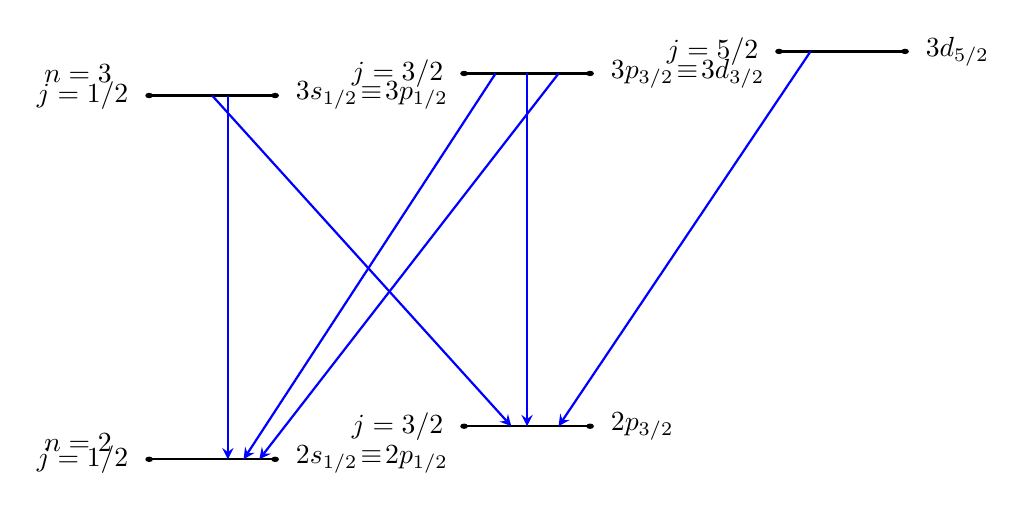
\begin{tikzpicture}[>=stealth, xscale=1.0, yscale=0.7]
  % n=3 levels
  \draw[thick] (0,7.6) -- (1.6,7.6);
  \node[left=4pt]  at (0,7.6) {$j=1/2$};
  \node[right=4pt] at (1.6,7.6) {$3s_{1/2}\!\equiv\!3p_{1/2}$};
  \draw[thick] (4.0,8.0) -- (5.6,8.0);
  \node[left=4pt]  at (4.0,8.0) {$j=3/2$};
  \node[right=4pt] at (5.6,8.0) {$3p_{3/2}\!\equiv\!3d_{3/2}$};
  \draw[thick] (8.0,8.4) -- (9.6,8.4);
  \node[left=4pt]  at (8.0,8.4) {$j=5/2$};
  \node[right=4pt] at (9.6,8.4) {$3d_{5/2}$};
  \node[left=10pt] at (0,8.0) {$n=3$};
  % n=2 levels
  \draw[thick] (0,1.0) -- (1.6,1.0);
  \node[left=4pt]  at (0,1.0) {$j=1/2$};
  \node[right=4pt] at (1.6,1.0) {$2s_{1/2}\!\equiv\!2p_{1/2}$};
  \draw[thick] (4.0,1.6) -- (5.6,1.6);
  \node[left=4pt]  at (4.0,1.6) {$j=3/2$};
  \node[right=4pt] at (5.6,1.6) {$2p_{3/2}$};
  \node[left=10pt] at (0,1.3) {$n=2$};
  % E1 transitions, downward
  \draw[->,thick,blue] (0.8,7.6) -- (4.6,1.6); % 3p_{1/2} -> 2p_{3/2}? actually 3p_{1/2} -> 2s_{1/2} below
  \draw[->,thick,blue] (1.0,7.6) -- (1.0,1.0); % 3s_{1/2}/3p_{1/2} -> 2s/2p_{1/2}
  \draw[->,thick,blue] (4.4,8.0) -- (1.2,1.0); % 3p_{3/2} -> 2s_{1/2}
  \draw[->,thick,blue] (4.8,8.0) -- (4.8,1.6); % 3p_{3/2}/3d_{3/2} -> 2p_{3/2}
  \draw[->,thick,blue] (5.2,8.0) -- (1.4,1.0); % 3d_{3/2} -> 2p_{1/2}
  \draw[->,thick,blue] (8.4,8.4) -- (5.2,1.6); % 3d_{5/2} -> 2p_{3/2}
  % marker dots at level ends
  \foreach \pt in {(0,7.6),(1.6,7.6),(4.0,8.0),(5.6,8.0),(8.0,8.4),(9.6,8.4),
                   (0,1.0),(1.6,1.0),(4.0,1.6),(5.6,1.6)}
    \fill \pt circle (1.4pt);
\end{tikzpicture}
\end{center}

E1 selection rules:
\begin{equation}
\Delta l=\pm 1,\quad\Delta s=0,\quad\Delta j=0,\pm 1\;(0\!\not\to\!0),\quad\Delta m_j=0,\pm 1.
\label{eq:E1-rules}
\end{equation}

\textit{Justification of $\Delta l=\pm 1$.} $\hat{\bm d}=-e\hat{\bm r}$ is a rank-1 odd-parity tensor. Parity selection forces $l-l'$ odd; Wigner--Eckart forces $|l-l'|\le 1$. Together: $\Delta l=\pm 1$.

\subsection*{(e) Doppler broadening at $T=\SI{300}{K}$}

Thermal Doppler FWHM:
\[
\frac{\Delta\nu_{\rm D}}{\nu_0}=\sqrt{\frac{8 k_{\rm B} T \ln 2}{M c^{2}}}.
\]
Insert $k_{\rm B}T\simeq\SI{4.14e-21}{J}$, $M=m_p$, $c^2\simeq\SI{9e16}{m^2 s^{-2}}$:
\[
\frac{\Delta\nu_{\rm D}^{\rm H}}{\nu_0}=\sqrt{\frac{8\cdot 4.14\!\times\!10^{-21}\!\cdot\!0.693}{1.67\!\times\!10^{-27}\cdot 9\!\times\!10^{16}}}.
\]
Evaluate:
\[
\frac{\Delta\nu_{\rm D}^{\rm H}}{\nu_0}\simeq 1.2\times 10^{-5}.
\]
He$^+$ has $M=4 m_p$, so width scales by $1/\sqrt{4}=1/2$:
\begin{equation}
\boxed{\;\frac{\Delta\nu_{\rm D}^{\rm H}}{\nu_0}\simeq 1.2\times 10^{-5},\qquad
\frac{\Delta\nu_{\rm D}^{\rm He^+}}{\nu_0}\simeq 6\times 10^{-6}.\;}
\label{eq:doppRes}
\end{equation}

\textit{Further mechanism in a discharge lamp.} Pressure (collisional) broadening: random collisional dephasing of the radiating dipole, Lorentzian width $\sim 1/\tau_{\rm coll}$. (Stark broadening from plasma microfields is also strong for H because of its linear Stark effect.)

\subsection*{(f) Fine structure equal to the H $2\to 3$ energy}

Equate $n=2,l=1$ splitting to $\tfrac{5}{36}hcR_\infty$:
\[
\frac{Z^{4}\alpha^{2}}{16}\,hcR_\infty=\frac{5}{36}\,hcR_\infty.
\]
Solve for $Z^4$:
\[
Z^{4}=\frac{80}{36\,\alpha^{2}}\simeq 4.2\times 10^{4}.
\]
\begin{equation}
\boxed{\;Z\simeq 14\;\;(\text{e.g.\ Si}^{13+}).\;}
\label{eq:Z-eq}
\end{equation}

\textit{Alkali $Z$-scaling.} Valence $np$ electron penetrates the unscreened core; SO coupling samples the bare nuclear field. Empirical $\Delta E_{\rm FS}$: Na \SI{0.42}{meV}, K \SI{2.0}{meV}, Rb \SI{6.96}{meV}, Cs \SI{28}{meV} — super-quartic in $Z$ because both the inner field and the penetrating-wavefunction amplitude grow with $Z$.

%==================================================================
\section*{Question 2 --- Hyperfine structure and the hydrogen MASER}
%==================================================================

\textbf{Problem.} Hamiltonian $\mathcal H=A\,\bm I\!\cdot\!\bm J+g_J\mu_{\rm B}\bm J\!\cdot\!\bm B-g_I\mu_N\bm I\!\cdot\!\bm B$. Identify each term, find the weak/strong-field crossover for ground-state H ($A/h=\SI{1420}{MHz}$, $I=1/2$), derive the eigenenergies in both regimes, and analyse a Stern--Gerlach beam with $B_z=\SI{1}{T}$, $\partial_z B_z=\SI{20}{T/m}$ as the basis of an H maser.

\subsection*{(a) Origin of each term}

$A\bm I\!\cdot\!\bm J$: hyperfine coupling of nuclear moment $\bm\mu_I=g_I\mu_N\bm I/\hbar$ to the electron-generated magnetic field at the nucleus (dominated by the Fermi-contact term for $s$ states).

$g_J\mu_{\rm B}\bm J\!\cdot\!\bm B$: electronic Zeeman, energy of $\bm\mu_J=-g_J\mu_{\rm B}\bm J/\hbar$ in $\bm B$.

$-g_I\mu_N\bm I\!\cdot\!\bm B$: nuclear Zeeman, smaller by $m_e/m_p\sim 1/1836$.

\textit{Regimes.} Weak field $g_J\mu_{\rm B}B\ll A$: $\bm I,\bm J$ couple to $\bm F=\bm I+\bm J$; good QNs $|F,m_F\rangle$. Strong field $g_J\mu_{\rm B}B\gg A$: $\bm I,\bm J$ decouple; good QNs $|m_J,m_I\rangle$ (Paschen--Back of hyperfine).

\subsection*{(b) Cross-over field}

Set $g_J\mu_{\rm B}B_c\simeq A$:
\[
A=h\cdot\SI{1420}{MHz}\simeq\SI{9.41e-25}{J}.
\]
With $g_J\simeq 2$ for the $1\,^2S_{1/2}$ ground state:
\[
B_c=\frac{A}{g_J\mu_{\rm B}}=\frac{\SI{9.41e-25}{J}}{2\cdot\SI{9.27e-24}{J/T}}.
\]
Evaluate:
\begin{equation}
\boxed{\;B_c\simeq\SI{50}{mT}\;(\sim\!500\,\mathrm{G}).\;}
\label{eq:Bc-est}
\end{equation}

\subsection*{(c) Weak-field eigenenergies}

Total spin $\bm F=\bm I+\bm J$, $\bm I\!\cdot\!\bm J=\tfrac{\hbar^2}{2}[F(F+1)-I(I+1)-J(J+1)]$.

For $I=J=1/2$, $F=0,1$:
\[
E_{F=1}^{(0)}=+\tfrac14 A\hbar^{2},\qquad E_{F=0}^{(0)}=-\tfrac34 A\hbar^{2}.
\]
Apply projection theorem within fixed $F$:
\[
\Braket{F m_F|J_z|F m_F}=\frac{F(F+1)+J(J+1)-I(I+1)}{2F(F+1)}\,m_F\hbar.
\]
Read off the Land\'e $g_F$:
\[
g_F=g_J\,\frac{F(F+1)+J(J+1)-I(I+1)}{2F(F+1)}-\frac{m_e}{m_p}\,g_I\,\frac{F(F+1)+I(I+1)-J(J+1)}{2F(F+1)}.
\]
Combine zero-field and Zeeman:
\begin{equation}
\boxed{\;E(F,m_F)=A\hbar^{2}\,\tfrac{F(F+1)-I(I+1)-J(J+1)}{2}+g_F\mu_{\rm B}B\,m_F\hbar.\;}
\label{eq:weak-field-E}
\end{equation}
For ground-state H: $g_{F=1}\simeq +1$, $g_{F=0}=0$ to leading order in $m_e/m_p$. Triplet splits linearly with $B$; singlet unshifted at first order.

\subsection*{(d) Strong-field eigenenergies}

In $|m_J,m_I\rangle$ Zeeman is diagonal. Decompose:
\[
\bm I\!\cdot\!\bm J=I_z J_z+\tfrac12(I_+J_-+I_-J_+).
\]
Drop ladder pieces (off-diagonal in the strong-field basis):
\[
\Braket{m_J,m_I|\bm I\!\cdot\!\bm J|m_J,m_I}=\hbar^2 m_J m_I.
\]
Add the Zeeman terms:
\[
E(m_J,m_I)=A\hbar^{2}m_J m_I+g_J\mu_{\rm B}B\,m_J\hbar-g_I\mu_N B\,m_I\hbar.
\]
Insert the four sign combinations:
\begin{align}
E_1=E(+\tfrac12,+\tfrac12)&=+\tfrac14 A\hbar^{2}+\tfrac12 g_J\mu_{\rm B}B\hbar-\tfrac12 g_I\mu_N B\hbar,\label{eq:strong1}\\
E_2=E(+\tfrac12,-\tfrac12)&=-\tfrac14 A\hbar^{2}+\tfrac12 g_J\mu_{\rm B}B\hbar+\tfrac12 g_I\mu_N B\hbar,\label{eq:strong2}\\
E_3=E(-\tfrac12,+\tfrac12)&=-\tfrac14 A\hbar^{2}-\tfrac12 g_J\mu_{\rm B}B\hbar-\tfrac12 g_I\mu_N B\hbar,\label{eq:strong3}\\
E_4=E(-\tfrac12,-\tfrac12)&=+\tfrac14 A\hbar^{2}-\tfrac12 g_J\mu_{\rm B}B\hbar+\tfrac12 g_I\mu_N B\hbar.\label{eq:strong4}
\end{align}
Stretched states $|\!\uparrow\Uparrow\rangle,|\!\downarrow\Downarrow\rangle$ ($|m_F|=1$) are exact eigenstates at all $B$; the $m_F=0$ pair is given exactly by Breit--Rabi.

\subsection*{(e) Forces and the H maser}

High-field upper states $E_1,E_2$ have $m_J=+1/2$; magnetic moment $\mu_z\simeq -\mu_{\rm B}$ (electron dominates). Force:
\[
F_z=-\frac{\partial E}{\partial z}=-(g_J\mu_{\rm B}m_J\hbar)\,\frac{\partial B_z}{\partial z}\mp(\tfrac12 g_I\mu_N\hbar)\,\frac{\partial B_z}{\partial z}.
\]
Take leading electronic piece, $g_J\mu_{\rm B}/2\simeq\mu_{\rm B}$, $m_{\rm H}\simeq m_p$:
\[
a\simeq\frac{\mu_{\rm B}}{m_p}\,\frac{\partial B_z}{\partial z}=\frac{\SI{9.27e-24}{J/T}}{\SI{1.67e-27}{kg}}\cdot\SI{20}{T/m}.
\]
Evaluate:
\begin{equation}
\boxed{\;|a|\simeq\SI{1.1e5}{m\,s^{-2}}\;\text{for both upper states.}\;}
\label{eq:accel}
\end{equation}

Fractional force difference set by nuclear Zeeman:
\[
\frac{\Delta F}{\langle F\rangle}\simeq\frac{g_I\mu_N}{g_J\mu_{\rm B}}\sim\frac{1}{1836}\sim 5\times 10^{-4}.
\]

\textit{Breit--Rabi connection.} Stretched states $|\!\uparrow\Uparrow\rangle,|\!\downarrow\Downarrow\rangle$ correspond to $|F=1,m_F=\pm 1\rangle$. The $m_F=0$ pair: $E_2$ at high field connects to $|F=1,m_F=0\rangle$; $E_3$ connects to $|F=0,m_F=0\rangle$.

\begin{center}
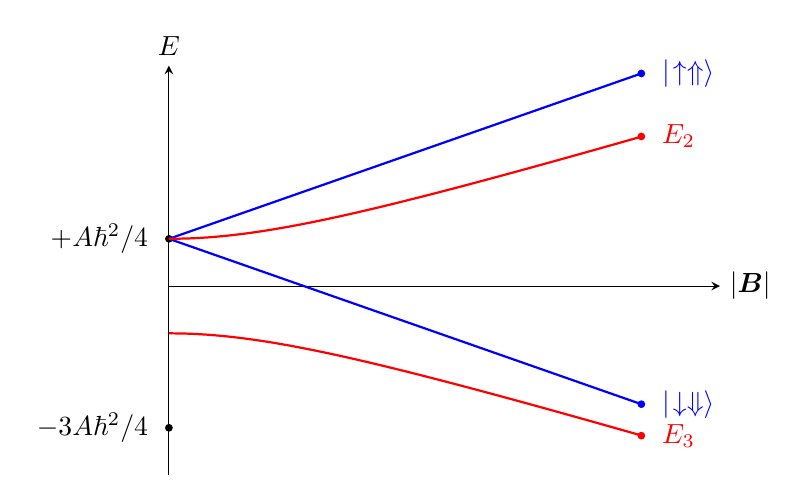
\begin{tikzpicture}[>=stealth, scale=1.0]
  \draw[->] (0,0) -- (7.0,0) node[right]{$|\bm B|$};
  \draw[->] (0,-2.4) -- (0,2.8) node[above]{$E$};
  % zero-field anchor
  \fill (0,0.6) circle (1.4pt);
  \fill (0,-1.8) circle (1.4pt);
  \node[left=4pt] at (0,0.6) {$+A\hbar^2/4$};
  \node[left=4pt] at (0,-1.8) {$-3A\hbar^2/4$};
  % m_F = +1 stretched: rises linearly
  \draw[thick,blue,domain=0:6,smooth,variable=\x] plot ({\x},{0.6+0.35*\x});
  \fill[blue] (6,2.7) circle (1.4pt);
  \node[blue,right=4pt] at (6,2.7) {$|\!\uparrow\Uparrow\rangle$};
  % m_F = -1 stretched: falls linearly
  \draw[thick,blue,domain=0:6,smooth,variable=\x] plot ({\x},{0.6-0.35*\x});
  \fill[blue] (6,-1.5) circle (1.4pt);
  \node[blue,right=4pt] at (6,-1.5) {$|\!\downarrow\Downarrow\rangle$};
  % m_F = 0 upper -> E_2: anticrosses upward
  \draw[thick,red,domain=0:6,smooth,variable=\x] plot ({\x},{0.6*sqrt(1+(\x/2)^2)});
  \fill[red] (6,1.9) circle (1.4pt);
  \node[red,right=4pt] at (6,1.9) {$E_2$};
  % m_F = 0 lower -> E_3
  \draw[thick,red,domain=0:6,smooth,variable=\x] plot ({\x},{-0.6*sqrt(1+(\x/2)^2)});
  \fill[red] (6,-1.9) circle (1.4pt);
  \node[red,right=4pt] at (6,-1.9) {$E_3$};
\end{tikzpicture}
\end{center}

\textit{Hydrogen maser.} The Stern--Gerlach gradient deflects low-field-seeking states $E_1,E_2$ ($m_J=+1/2$) into a PTFE-coated storage bulb. Inside a low-field microwave cavity tuned to $\nu_{\rm hf}=\SI{1420}{MHz}$, only the upper $F=1$ levels are populated, the $|F=0,m_F=0\rangle$ ground-hyperfine state is empty, and the $\Delta F=1,\Delta m_F=0$ M1 transition is driven by stimulated emission. Wall-collision lifetimes of $\sim\!\si{s}$ give an extremely narrow Lorentzian and a precision frequency standard.

%==================================================================
\section*{Question 3 --- Three- vs.\ four-level lasers and the Yb fibre}
%==================================================================

\textbf{Problem.} (a) Threshold contrast between three- and four-level systems. (b) Derive the gain coefficient from the Einstein relations. (c)--(g) Yb-doped fibre: $r=\SI{2}{\micro m}$, $L=\SI{0.5}{m}$, $\sigma_{\rm abs}=\SI{6e-25}{m^2}$, $\sigma_{\rm em}=\SI{2.5e-25}{m^2}$, $86\%$ pump absorption at \SI{910}{nm}, lower-band sublevels at $E_{1A}/hc=\SI{60000}{m^{-1}}$, $E_{1B}/hc=\SI{106000}{m^{-1}}$, upper level at $\SI{1026000}{m^{-1}}$.

\subsection*{(a) Threshold for three- vs.\ four-level lasers}

Inversion $N^*=N_2-(g_2/g_1)N_1$ must overcome cavity loss.

Four-level: $|1\rangle$ above the ground state, thermally empty ($N_1\sim e^{-\Delta E/k_{\rm B}T}\to 0$); inversion needs an infinitesimal fraction of ground population pumped.

Three-level: $|1\rangle$ is the ground state; need $N_2>N_1$, i.e.\ $>\!\tfrac12$ of all ions pumped. Threshold pump rate $\sim$ spontaneous-decay rate $\times\,N/2$, orders of magnitude larger.

\subsection*{(b) Gain coefficient}

Rate equation for a beam of intensity $I$, lineshape $g(\nu-\nu_0)$, in the unsaturated regime:
\[
\frac{\de I}{\de z}=\frac{\hbar\omega_0}{c}\,g(\nu-\nu_0)\,(B_{21}N_2-B_{12}N_1)\,I.
\]
Assumptions: (i) plane wave; (ii) homogeneous broadening, $\int g\,\de\nu=1$; (iii) populations not depleted; (iv) thermal photons negligible at optical frequency.

Define $\gamma(\nu)$ by $\de I/\de z=\gamma I$:
\[
\gamma(\nu)=\frac{\hbar\omega_0\,g(\nu-\nu_0)}{c}\,(B_{21}N_2-B_{12}N_1).
\]
Apply $g_1 B_{12}=g_2 B_{21}$:
\[
\gamma(\nu)=\frac{\hbar\omega_0\,g(\nu-\nu_0)}{c}\,B_{21}\!\left[N_2-\frac{g_2}{g_1}N_1\right].
\]
Eliminate $B_{21}$ via $A_{21}=\hbar\omega_0^{3}B_{21}/(\pi^{2}c^{3})$:
\begin{equation}
\boxed{\;\gamma(\nu)=\frac{\pi^{2}c^{2}A_{21}}{\omega_0^{2}}\,g(\nu-\nu_0)\!\left[N_2-\frac{g_2}{g_1}N_1\right]=\sigma_{\rm em}(\nu)\,N^{*}.\;}
\label{eq:gain-final}
\end{equation}

\subsection*{(c) Yb ion density}

Beer absorption: $I(L)/I(0)=e^{-\sigma_{\rm abs}NL}=0.14$ ($86\%$ absorbed):
\[
\sigma_{\rm abs}\,N\,L=-\ln 0.14=1.97.
\]
Solve for $N$:
\[
N=\frac{1.97}{\SI{6e-25}{m^2}\cdot\SI{0.5}{m}}.
\]
Evaluate:
\begin{equation}
\boxed{\;N\simeq\SI{6.6e24}{m^{-3}}.\;}
\label{eq:N-yb}
\end{equation}

\subsection*{(d) Lower-band thermal populations at \SI{300}{K}}

Boltzmann factors with $g_0=g_{1A}=g_{1B}=1$. At $T=\SI{300}{K}$, $k_{\rm B}T/hc\simeq\SI{2.084e4}{m^{-1}}$:
\[
\frac{E_{1A}}{k_{\rm B}T}=\frac{60\,000}{2.084\!\times\!10^{4}}\simeq 2.88,\quad
\frac{E_{1B}}{k_{\rm B}T}=\frac{106\,000}{2.084\!\times\!10^{4}}\simeq 5.09.
\]
Partition sum:
\[
Z_{\rm low}=1+e^{-2.88}+e^{-5.09}=1+0.0561+0.00614\simeq 1.062.
\]
Fractional populations $f_\alpha=e^{-E_\alpha/k_{\rm B}T}/Z_{\rm low}$:
\begin{equation}
\boxed{\;f_{1A}\simeq 5.3\times 10^{-2},\qquad f_{1B}\simeq 5.8\times 10^{-3}.\;}
\label{eq:frac-low}
\end{equation}

\subsection*{(e) Threshold pump energies}

Threshold: $N_{2,\rm th}=N_{1\alpha}\simeq f_{1\alpha}(N-N_2)\simeq f_{1\alpha}N$ ($f_{1\alpha}\ll 1$).

Pump-photon energy:
\[
E_{\rm pump}=\frac{hc}{\SI{910e-9}{m}}\simeq\SI{2.18e-19}{J}\simeq\SI{1.36}{eV}.
\]
Core volume:
\[
V=\pi r^{2}L=\pi(\SI{2e-6}{m})^{2}\cdot\SI{0.5}{m}\simeq\SI{6.28e-12}{m^{3}}.
\]
Total ions:
\[
NV\simeq\SI{6.6e24}{m^{-3}}\cdot\SI{6.28e-12}{m^{3}}\simeq 4.14\times 10^{13}.
\]
Threshold pump energy $E_{\alpha,\rm th}=f_{1\alpha}NV E_{\rm pump}$:
\[
E_{A,\rm th}=5.3\times 10^{-2}\cdot 4.14\times 10^{13}\cdot\SI{2.18e-19}{J}.
\]
\[
E_{B,\rm th}=5.8\times 10^{-3}\cdot 4.14\times 10^{13}\cdot\SI{2.18e-19}{J}.
\]
Evaluate:
\begin{equation}
\boxed{\;E_{A,\rm th}\simeq\SI{0.48}{\micro J},\qquad E_{B,\rm th}\simeq\SI{52}{nJ}.\;}
\label{eq:Eth-results}
\end{equation}

\subsection*{(f) Round-trip gain at $E=5E_{B,\rm th}$}

Excited density:
\[
N_2=5 f_{1B}N=5\cdot 5.8\times 10^{-3}\cdot\SI{6.6e24}{m^{-3}}\simeq\SI{1.9e23}{m^{-3}}.
\]
Lower-band populations of remaining ions:
\[
N_{1A}\simeq f_{1A}(N-N_2)\simeq\SI{3.4e23}{m^{-3}},\qquad N_{1B}\simeq f_{1B}(N-N_2)\simeq\SI{3.7e22}{m^{-3}}.
\]
Inversions ($g_2/g_{1\alpha}=1$):
\[
N^{*}_{A}=\SI{1.9e23}{m^{-3}}-\SI{3.4e23}{m^{-3}}\simeq -\SI{1.5e23}{m^{-3}}<0.
\]
\[
N^{*}_{B}=\SI{1.9e23}{m^{-3}}-\SI{3.7e22}{m^{-3}}\simeq +\SI{1.5e23}{m^{-3}}.
\]
Round-trip gain on $2\to 1B$:
\[
G_{\rm rt}=\exp(2\sigma_{\rm em}N^{*}_{B}L)=\exp(2\cdot\SI{2.5e-25}{m^2}\cdot\SI{1.5e23}{m^{-3}}\cdot\SI{0.5}{m}).
\]
Evaluate the exponent:
\[
2\sigma_{\rm em}N^{*}_{B}L=3.75\times 10^{-2}.
\]
\begin{equation}
\boxed{\;G_{\rm rt}\simeq e^{0.038}\simeq 1.04\;(\sim 4\%);\;\text{no gain on }2\!\to\!1A.\;}
\label{eq:Grt-num}
\end{equation}

\subsection*{(g) Maximum efficiency and losses}

Quantum-defect efficiency:
\[
\eta_{\rm QD}=\frac{\lambda_{\rm pump}}{\lambda_{\rm laser}}=\frac{E_{\rm laser}}{E_{\rm pump}}.
\]
$2\to 1B$: $E_{\rm laser}/hc=(1\,026\,000-106\,000)\,\si{m^{-1}}=920\,000\,\si{m^{-1}}$, $E_{\rm pump}/hc=1\,099\,000\,\si{m^{-1}}$:
\[
\eta_{\rm QD}^{B}=\frac{920}{1099}\simeq 0.837.
\]
$2\to 1A$: $E_{\rm laser}/hc=966\,000\,\si{m^{-1}}$:
\[
\eta_{\rm QD}^{A}=\frac{966}{1099}\simeq 0.879.
\]
Combine with $\eta_{\rm diode}=0.60$ and $\eta_{\rm abs}=0.86$:
\[
\eta_{\rm max}^{B}=0.60\cdot 0.86\cdot 0.837\simeq 0.43.
\]
\[
\eta_{\rm max}^{A}\simeq 0.60\cdot 0.86\cdot 0.879\simeq 0.45.
\]
\begin{equation}
\boxed{\;\eta_{\rm max}\simeq 43\text{--}45\%.\;}
\label{eq:eta-max}
\end{equation}

\textit{Practical losses.} Ground-state absorption on the laser line (especially $2\to 1B$, quasi-three-level); excited-state absorption from level $2$; non-radiative quenching by impurities or Yb clusters; cavity scattering; sub-optimal output coupling; pump-heating broadening of the emission line.

%==================================================================
\section*{Question 4 --- Radiative transfer and lithium absorption}
%==================================================================

\textbf{Problem.} Recast $\de I_\nu/\de z=-\alpha_\nu I_\nu+j_\nu$ in optical-depth form, solve for constant $S_\nu$, and use measured ratios $I_A:I_B:I_C=0.85:1:0.15$ to extract $\tau_\nu$ and $S_\nu/I_\nu(0)$. Show $\sigma_{\rm abs}^{\rm res}=\lambda_0^2/(2\pi)$ for a lifetime-broadened line, evaluate for Li $2s\to 2p$ at \SI{671}{nm}, give the column density for $\tau\sim 1$ in a \SI{1}{cm} cell, and discuss when natural-width lines are observed; list the source requirements for the Li $2s\to np$ Rydberg series.

\subsection*{(a) Optical-depth form and formal solution}

Define:
\[
\de\tau_\nu=\alpha_\nu\,\de z,\qquad S_\nu=\frac{j_\nu}{\alpha_\nu}.
\]
Divide transfer equation by $\alpha_\nu$:
\[
\frac{\de I_\nu}{\de\tau_\nu}=-I_\nu+S_\nu.
\]
Multiply by integrating factor $e^{\tau_\nu}$:
\[
\frac{\de}{\de\tau_\nu}\!\left(I_\nu e^{\tau_\nu}\right)=S_\nu e^{\tau_\nu}.
\]
Integrate from $0$ to $\tau_\nu$ at constant $S_\nu$:
\[
I_\nu(\tau_\nu)e^{\tau_\nu}-I_\nu(0)=S_\nu(e^{\tau_\nu}-1).
\]
Solve for $I_\nu$:
\begin{equation}
\boxed{\;I_\nu(\tau_\nu)=I_\nu(0)e^{-\tau_\nu}+S_\nu(1-e^{-\tau_\nu}).\;}
\label{eq:RTsol}
\end{equation}
Beer's law in the limit $\tau_\nu\to 0$; black-body $S_\nu$ in the limit $\tau_\nu\to\infty$.

\subsection*{(b) Inversion of the flame measurement}

Identify the three measurements with \eqref{eq:RTsol}:
\[
I_A=I_\nu(0)e^{-\tau_\nu}+S_\nu(1-e^{-\tau_\nu}),\quad I_B=I_\nu(0),\quad I_C=S_\nu(1-e^{-\tau_\nu}).
\]
Subtract $I_C$ from $I_A$:
\[
I_A-I_C=I_B\,e^{-\tau_\nu}.
\]
Divide by $I_B$, set $X=I_A/I_B,Y=I_C/I_B$:
\[
e^{-\tau_\nu}=X-Y=0.85-0.15=0.70.
\]
Take log:
\begin{equation}
\boxed{\;\tau_\nu=-\ln 0.70\simeq 0.357.\;}
\label{eq:tau-num}
\end{equation}
Read $S_\nu/I_\nu(0)$ from $I_C$:
\[
\frac{S_\nu}{I_\nu(0)}=\frac{Y}{1-e^{-\tau_\nu}}=\frac{0.15}{1-0.70}.
\]
Evaluate:
\begin{equation}
\boxed{\;\frac{S_\nu}{I_\nu(0)}=0.50.\;}
\label{eq:S-num}
\end{equation}
Optically thin flame; carbon emits with half the incoming black-body brightness at this frequency.

\subsection*{(c) Resonant cross section and the Li $2s\to 2p$ line}

Lifetime-limited Lorentzian, $\Gamma=A_{21}$:
\[
g_L(\omega-\omega_0)=\frac{1}{2\pi}\,\frac{\Gamma}{(\omega-\omega_0)^{2}+(\Gamma/2)^{2}}.
\]
Evaluate on resonance:
\[
g_L(0)=\frac{2}{\pi A_{21}}.
\]
Insert in $\sigma_{\rm abs}=(g_2/g_1)(\pi^2 c^2 A_{21}/\omega_0^2)\,g_L$, take $g_2/g_1=1$:
\[
\sigma_{\rm abs}^{\rm res}=\frac{\pi^{2}c^{2}A_{21}}{\omega_0^{2}}\cdot\frac{2}{\pi A_{21}}=\frac{2\pi c^{2}}{\omega_0^{2}}.
\]
Use $\omega_0=2\pi c/\lambda_0$:
\begin{equation}
\boxed{\;\sigma_{\rm abs}^{\rm res}=\frac{\lambda_0^{2}}{2\pi}\;\;\text{(independent of }A_{21}).\;}
\label{eq:sigma-res}
\end{equation}

For Li, $\lambda_0=\SI{671}{nm}$:
\[
\sigma_{\rm abs}^{\rm res}=\frac{(\SI{671e-9}{m})^{2}}{2\pi}\simeq\SI{7.2e-14}{m^{2}}.
\]
\begin{equation}
\boxed{\;\sigma_{\rm abs}^{\rm res}\simeq\SI{7e-14}{m^{2}}.\;}
\label{eq:sigma-Li}
\end{equation}

Column density for $\tau\sim 1$ at $L=\SI{1}{cm}$:
\[
N\sim\frac{1}{\sigma_{\rm abs}^{\rm res}L}=\frac{1}{\SI{7.2e-14}{m^2}\cdot\SI{e-2}{m}}.
\]
Evaluate:
\begin{equation}
\boxed{\;N_{\rm Li}\sim\SI{1.4e15}{m^{-3}}\;(\sim 10^{9}\,\mathrm{cm^{-3}}).\;}
\label{eq:N-thick}
\end{equation}

\textit{When are pure lifetime-broadened lines seen?} Natural width must dominate Doppler ($\propto\sqrt{T/M}$) and pressure ($\propto N\sigma_{\rm coll}\bar v$) widths: very low temperature (laser cooling, transverse atomic beams with $\bm k\!\cdot\!\bm v\to 0$), very low pressure ($\tau_{\rm coll}\gg\tau_{\rm rad}$), and absence of inhomogeneous mechanisms (Stark, transit-time). Examples: forbidden lines via saturated absorption, Ramsey spectroscopy, single-ion traps.

\subsection*{(d) Source for the $2s\to np$ Li series}

Li ground state $1s^{2}2s$, ionisation $\SI{5.39}{eV}\equiv\SI{43484}{cm^{-1}}$, series limit $\lambda_{\rm lim}\simeq\SI{230}{nm}$.

Required source properties:

(i) \textit{Continuum coverage} from $\sim\SI{671}{nm}$ down to $\sim\SI{230}{nm}$: D$_2$ arc, Xe arc, tungsten + UV continuum, or synchrotron radiation, so absorption appears as dips on a smooth background.

(ii) \textit{High UV brightness}: peak cross section $\propto 1/n^{*5}$ for high Rydberg states; need adequate UV signal-to-noise.

(iii) \textit{Featureless/stable spectrum}: any source structure mimics absorption; alternative is a swept tunable laser of sufficient range.

(iv) \textit{Resolving power} $\Delta\nu/\nu\lesssim 10^{-6}$ to resolve Doppler width at $T\sim\SI{700}{K}$: Echelle, Fourier-transform, or two-photon Doppler-free laser spectroscopy.

(v) \textit{Long-term intensity stability}: faint high-$n$ lines need steady $I/I_0$ ratios over long acquisition.

In short: continuum or broadly tunable laser covering $230\text{--}\SI{700}{nm}$, high UV brightness, excellent stability, recorded at high resolving power against a wavelength reference.

\end{document}
